\documentclass[tikz,border=12pt]{standalone}
% Shared visual language for standalone EMT block diagrams.
\usepackage{amsmath}
\usetikzlibrary{arrows.meta,backgrounds,calc,fit,positioning}

\tikzset{
    emt diagram/.style = {>={Stealth[length=2.4mm]}},
    line/.style        = {semithick, rounded corners=6pt},
    block/.style       = {draw, semithick, fill=white,
                          minimum height=1cm, minimum width=2.3cm},
    hblock/.style      = {block, minimum width=2.24cm, minimum height=1.3cm},
    vblock/.style      = {block, minimum width=1.3cm, minimum height=2.24cm},
    sum/.style         = {draw, semithick, fill=white, circle,
                          inner sep=2.6pt},
    signal/.style      = {circle, fill, inner sep=1.4pt,
                          label distance=3pt},
    sig/.style         = {font=\small},
    pm/.style          = {font=\scriptsize},
    wire jump/.style   = {line,
                          preaction={draw=white, line width=3pt,
                                     line cap=round}},
    enclosure/.style   = {draw, dashed, semithick, rounded corners=4pt},
    operator enclosure/.style = {enclosure, inner xsep=7mm, inner ysep=6mm}
}


\begin{document}
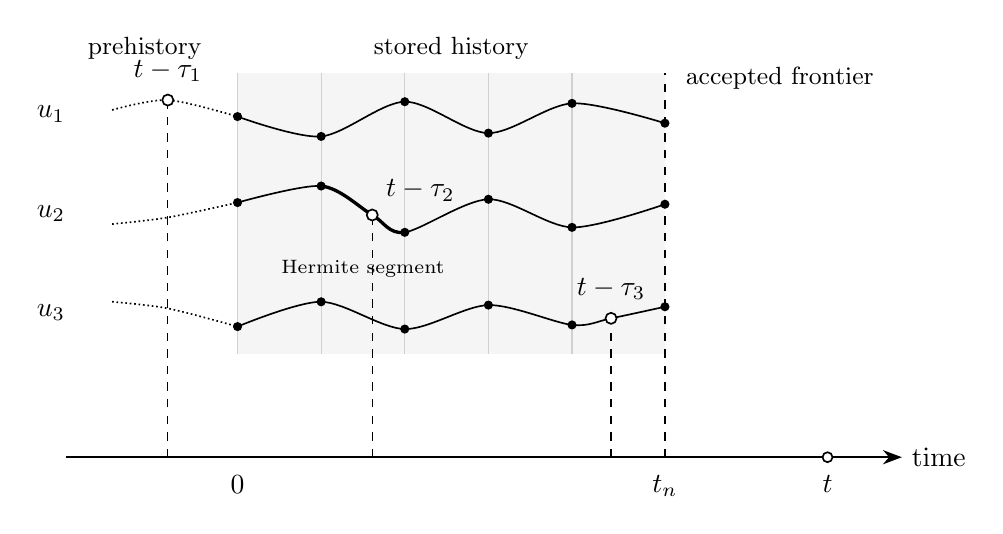
\begin{tikzpicture}[emt diagram, x=1.18cm, y=1.05cm]

% Stored history and its shared knot times
\fill[black!4] (2.0,1.25) rectangle (6.6,4.65);
\foreach \x in {2.0,2.9,3.8,4.7,5.6}
    \draw[black!18, thin] (\x,1.25) -- (\x,4.65);
\draw[dashed, semithick] (6.6,0) -- (6.6,4.65);

% Time axis and region labels
\draw[->, line] (0.15,0) -- (9.15,0) node[right] {time};
\node[below=3pt] at (2.0,0) {$0$};
\node[below=3pt] at (6.6,0) {$t_n$};
\draw[fill=white, semithick] (8.35,0) circle (1.8pt);
\node[below=3pt] at (8.35,0) {$t$};
\node[font=\small] at (1.0,4.95) {prehistory};
\node[font=\small] at (4.3,4.95) {stored history};
\node[font=\small, anchor=west] at (6.72,4.58) {accepted frontier};

% Channel 1: the lookup lies in the analytic prehistory
\node[left] at (0.25,4.15) {$u_1$};
\draw[densely dotted, semithick]
    plot[smooth] coordinates {
      (0.65,4.2) (1.25,4.32) (2.0,4.12)
    };
\draw[semithick]
    plot[smooth] coordinates {
      (2.0,4.12) (2.9,3.88) (3.8,4.3) (4.7,3.92)
      (5.6,4.28) (6.6,4.04)
    };
\foreach \x/\y in {2.0/4.12,2.9/3.88,3.8/4.3,4.7/3.92,5.6/4.28,6.6/4.04}
    \fill (\x,\y) circle (1.65pt);
\draw[dashed, thin] (1.25,0) -- (1.25,4.32);
\draw[fill=white, semithick] (1.25,4.32) circle (2pt)
    node[above=3pt] {$t-\tau_1$};

% Channel 2: lookup within a Hermite segment
\node[left] at (0.25,2.95) {$u_2$};
\draw[densely dotted, semithick]
    plot[smooth] coordinates {
      (0.65,2.82) (1.25,2.9) (2.0,3.08)
    };
\draw[semithick]
    plot[smooth] coordinates {
      (2.0,3.08) (2.9,3.28) (3.45,2.93) (3.8,2.72)
      (4.7,3.12) (5.6,2.78) (6.6,3.06)
    };
\begin{scope}
    \clip (2.9,2.55) rectangle (3.8,3.4);
    \draw[very thick]
        plot[smooth] coordinates {
          (2.0,3.08) (2.9,3.28) (3.45,2.93) (3.8,2.72) (4.7,3.12)
        };
\end{scope}
\foreach \x/\y in {2.0/3.08,2.9/3.28,3.8/2.72,4.7/3.12,5.6/2.78,6.6/3.06}
    \fill (\x,\y) circle (1.65pt);
\draw[dashed, thin] (3.45,0) -- (3.45,2.93);
\draw[fill=white, semithick] (3.45,2.93) circle (2pt)
    node[above right=2pt] {$t-\tau_2$};
\node[font=\scriptsize, anchor=north] at (3.35,2.5) {Hermite segment};

% Channel 3: the shallowest lookup remains behind the frontier
\node[left] at (0.25,1.75) {$u_3$};
\draw[densely dotted, semithick]
    plot[smooth] coordinates {
      (0.65,1.88) (1.25,1.8) (2.0,1.58)
    };
\draw[semithick]
    plot[smooth] coordinates {
      (2.0,1.58) (2.9,1.88) (3.8,1.55) (4.7,1.84)
      (5.6,1.6) (6.02,1.68) (6.6,1.82)
    };
\foreach \x/\y in {2.0/1.58,2.9/1.88,3.8/1.55,4.7/1.84,5.6/1.6,6.6/1.82}
    \fill (\x,\y) circle (1.65pt);
\draw[dashed, thin] (6.02,0) -- (6.02,1.68);
\draw[fill=white, semithick] (6.02,1.68) circle (2pt)
    node[above=3pt] {$t-\tau_3$};

\end{tikzpicture}
\end{document}
